% Copyright 2010 by Frank Wood

\documentclass{beamer}
\usepackage{algorithm}
\usepackage{algorithmic}
\usepackage[numbers]{natbib}

% Setup appearance:

\usetheme{Darmstadt}
\usefonttheme[onlylarge]{structurebold}
\setbeamerfont*{frametitle}{size=\normalsize,series=\bfseries}
\setbeamertemplate{navigation symbols}{}

% Standard packages

\usepackage[english]{babel}
%\usepackage[latin1]{inputenc}
%\usepackage{times}
%\usepackage[T1]{fontenc}
%\usepackage{nnfootnote}
\usepackage{amsfonts}
\usepackage{amsmath}
%\newcommand{\argmax}{\operatornamewithlimits{argmax}}
\def\newblock{\hskip .11em plus .33em minus .07em}
% Setup TikZ

%\usepackage{tikz}
%\usetikzlibrary{arrows}
%\tikzstyle{block}=[draw opacity=0.7,line width=1.4cm]


% Author, Title, etc.

\title[Applied Bayesian Nonparametrics] 
{
  Applied Bayesian Nonparametrics
}

\author[Wood]
{
  Frank~Wood%\inst{1}
}

\institute[Columbia University]
{
  %\inst{1}%
  Columbia University
}

\date[Job Talk 2010]
{Job Talk 2010}

%\def\blfootnote{\xdef\@thefnmark{}\@footnotetext}


% The main document
% !TEX root = talk.tex

\newcommand{\comment}[1]{}
%\newcommand{\comment}[1]{{\marginpar{\tiny {#1} }}}
\def\todo#1{TODO(#1)}

\def\bigO{{\mathcal O}}
\def\balpha{\mbox{\boldmath $\alpha$}}
\def\bbeta{\mbox{\boldmath $\beta$}}
\def\beeta{\mbox{\boldmath $\eta$}}
\def\blambda{\mbox{\boldmath $\lambda$}}
\def\bmu{\mbox{\boldmath $\mu$}}
\def\bphi{\mbox{\boldmath $\phi$}}
\def\bpsi{\mbox{\boldmath $\psi$}}
\def\bsigma{\mbox{\boldmath $\sigma$}}
\def\btau{\mbox{\boldmath $\tau$}}
\def\btheta{\mbox{\boldmath $\theta$}}
\def\dbphi{\dot{\mbox{\boldmath $\phi$}}}
\def\dbtau{\dot{\mbox{\boldmath $\tau$}}}
\def\dbtheta{\dot{\mbox{\boldmath $\theta$}}}

%\newcommand{\nofootnotemark}{\let\@makefnmark\relax}
\newcommand{\bX}{\mathbf{X}}
\newcommand{\bY}{\mathbf{Y}}
\newcommand{\bW}{\mathbf{W}}
\newcommand{\bZ}{\mathbf{Z}}
\newcommand{\bH}{\mathbf{H}}
\newcommand{\bQ}{\mathbf{Q}}
\newcommand{\bA}{\mathbf{A}}
\newcommand{\bI}{\mathbf{I}}
\newcommand{\by}{\mathbf{y}}
\newcommand{\bz}{\mathbf{z}}
\newcommand{\bx}{\mathbf{x}}

\newcommand{\ith}{i^\mathrm{th}}
\def\A{{\bf A}}
\def\B{{\bf B}}
\def\C{{\bf C}}
\def\D{{\bf D}}
\def\F{{\bf F}}
\def\L{{\bf L}}
\def\M{{\bf M}}
\def\W{{\bf W}}
\def\I{{\bf I}}
\def\J{{\bf J}}
\def\R{{\bf R}}
\def\U{{\bf U}}
\def\V{{\bf V}}
\def\b{{\bf b}}
\def\c{{\bf c}}
\def\d{{\bf d}}
\def\r{{\bf r}}
\def\s{{\bf s}}
\def\t{{\bf t}}
\def\u{{\bf u}}
\def\v{{\bf v}}
\def\f{{\bf f}}
\def\x{{\bf x}}
\def\y{{\bf y}}
\def\w{{\bf w}}
\def\vo{{\bf o}}
\def\p{{\bf p}}
\def\O{{\bf 0}}
%\def\a{{\bf a}}


\def\vbpsi{\vec{\mbox{\boldmath $\psi$}}} 
\def\vpsi{\vec{\psi}} 
\def\vbphi{\vec{\mbox{\boldmath $\phi$}}} 
\def\vphi{\vec{\phi}} 
\def\vbtau{\vec{\mbox{\boldmath $\tau$}}} 
\def\vbtheta{\vec{\mbox{\boldmath $\theta$}}} 
\def\vD{\vec{D}}
\def\vf{\vec{\bf f}}
\def\vF{\vec{\bf F}}
\def\vI{\vec{\bf I}}
\def\vR{\vec{\bf R}}
\def\vv{\vec{v}}
\def\vV{\vec{\bf V}}

\def\pon{p_{\mathrm{on}}}
\def\poff{p_{\mathrm{off}}}

\def\tr{^{\text{T}}}

%%% Vector notation for sections 3 and 4
%%% Vector notation for sections 3 and 4
\def\mvec{\vec{m}}
\def\fvec{\vec{f}}
\def\appfvec{\vec{f}_k}
\def\avec{\vec{a}}
\def\bvec{\vec{b}}
\def\evec{\vec{e}}
\def\uvec{\vec{u}}
\def\xvec{\vec{x}}
\def\wvec{\vec{w}}
\def\gradvec{\vec{\nabla}}

\def\aM{\mbox{\bf a}_M}
\def\aS{\mbox{\bf a}_S}
\def\aO{\mbox{\bf a}_O}
\def\aL{\mbox{\bf a}_L}
\def\aP{\mbox{\bf a}_P}
\def\ai{\mbox{\bf a}_i}
\def\aj{\mbox{\bf a}_j}
\def\an{\mbox{\bf a}_n}
\def\a1{\mbox{\bf a}_1}
\def\a2{\mbox{\bf a}_2}
\def\a3{\mbox{\bf a}_3}
\def\a4{\mbox{\bf a}_4}

%\def\x{\mbox{\bf x\/}}
%\def\X{\mbox{\bf X}}
%\def\A{\mbox{\bf A}}
%\def\P{\mbox{\bf P}}
%\def\C{\mbox{\bf C}}
%\def\c{\mbox{\bf c}}
%\def\b{\mbox{\bf b}}
%\def\o{\mbox{\bf o}}
%\def\h{\mbox{\bf h}}
%\def\f{\mbox{\bf f}}
%\def\x{\mbox{\bf x}}
%\def\sx{\mbox{\scriptsize\bf x}}
%\def\z{\mbox{\bf z}}
%\def\l{\mbox{\bf l}}
%\def\m{\mbox{\bf m}}
%\def\bi{\mbox{\bf i}}
%\def\u{\mbox{\bf u}}
%\def\v{\mbox{\bf v}}
\def\a{\mbox{\bf a}}
%\def\p{\mbox{\bf p}}
%\def\r{\mbox{\bf r}}
%\def\d{\mbox{\bf d}}
%\def\Q{\mbox{\bf Q}}
%\def\s{\mbox{\bf s}}
%\def\st{\mbox{\scriptsize\bf t}}
%\def\ss{\mbox{\scriptsize\bf s}}
%\def\t{\mbox{\bf t}}
%\def\cR{{\cal R}}
%\def\calD{{\cal D}}
%\def\calS{{\cal S}}
%\def\g{\mbox{\bf g}}
%\def\e{\mbox{\bf e}}
%\def\flow{\{\mbox{\bf u}\}}
%\def\appearChange{iconic change}

\def\sigmae{\sigma}
\def\sigmam{\sigma}

\newcommand{\eg}{e.\thinspace{}g.,\@\xspace}
\newcommand{\egn}{e.\thinspace{}g.\@\xspace}
\newcommand{\cf}{cf.\@\xspace}
\newcommand{\ie}{i.\thinspace{}e.,\@\xspace}
\newcommand{\ien}{i.\thinspace{}e.\@\xspace}
\newcommand{\iid}{i.\thinspace{}i.\thinspace{}d.\@\xspace}


%\newcommand{\comment}[1]{}
\newcommand{\ponedec}{\mathcal{P}^\downarrow_1}
\newcommand{\pone}{\mathcal{P}_1}
\newcommand{\rank}[1]{\mathrm{RANK}\left[#1\right]}
\newcommand{\E}[1]{\mathrm{E}\left[#1\right]}
%\newcommand{\PY}{\mathcal{PY}}
%\newcommand{\DP}{\mathcal{DP}}
%\newcommand{\iid}{iid.}
\newcommand{\drawiid}{\stackrel{\text{iid}}{\sim}}
\newcommand{\vect}[1]{\mathbf{#1}}
\newcommand{\indicator}[1]{\text{I}\left[ #1 \right]}
\newcommand{\pdcoag}{PD(d_1,0)-\text{COAG}}
%\newcommand{\todo}{\textbf{*TODO*}}
\newcommand{\igram}{\text{$\infty$-gram}}
\newcommand{\Prob}{\text{P}}

\def\mm{sequence memoizer }
\def\MM{SM }

\def\pibf{{\boldsymbol{\pi}}}
\def\kapbf{\boldsymbol{\kappa}}
\def\taubf{\boldsymbol{\tau}}
\def\thebf{\boldsymbol{\theta}}
\def\rhobf{\boldsymbol{\rho}}
\def\phibf{\boldsymbol{\phi}}
\def\pbf{\mathbf{p}}
\def\qbf{\mathbf{q}}
\def\sbf{\mathbf{s}}
\def\tbf{\mathbf{t}}
\def\ybf{\mathbf{y}}
\def\ubf{\mathbf{u}}
\def\Ave{\mathbb{E}}

\def\wbf{\mathbf{w}}
\def\xbf{\mathbf{x}}
\def\rbf{\mathbf{r}}
\def\tbf{\mathbf{t}}
\def\kbf{\mathbf{k}}
\def\Xbf{\mathbf{X}}
\def\0bf{\mathbf{0}}
\def\Ibf{\mathbf{I}}
\def\phibf{\mathbf{\phi}}
\def\Phibf{\mathbf{\Phi}}
\def\disteq{{\stackrel{D}{=}}}
\def\EE{{\mathbb{E}}}
\def\GG{\mathcal{G}}
\def\G{G}
\def\U{U}

\def\phiv{\varphi}
\def\phivbf{\boldsymbol{\varphi}}

\def\Ocal{\mathcal{O}}
\DeclareMathOperator*{\Var}{Var}

\DeclareMathOperator*{\Bet}{Beta}
\DeclareMathOperator{\coag}{COAG}
\DeclareMathOperator{\frag}{FRAG}
\DeclareMathOperator*{\rnk}{RANK}
\DeclareMathOperator*{\gem}{GEM}
\DeclareMathOperator*{\pd}{PD}
\DeclareMathOperator*{\py}{PY}
\DeclareMathOperator*{\DP}{DP}
\DeclareMathOperator*{\PY}{PY}
\DeclareMathOperator*{\gd}{GDir}
\DeclareMathOperator*{\Dir}{Dir}
\DeclareMathOperator*{\CRP}{CRP}
\DeclareMathOperator*{\argmax}{argmax}



%%% Local Variables: 
%%% mode: latex
%%% TeX-master: "paper"
%%% End: 
% !TEX root = talk.tex
%
%\newcommand{\comment}[1]{}
%%\newcommand{\comment}[1]{{\marginpar{\tiny {#1} }}}
%
%\def\bigO{{\mathcal O}}
%\def\balpha{\mbox{\boldmath $\alpha$}}
%\def\bbeta{\mbox{\boldmath $\beta$}}
%\def\beeta{\mbox{\boldmath $\eta$}}
%\def\blambda{\mbox{\boldmath $\lambda$}}
%\def\bmu{\mbox{\boldmath $\mu$}}
%\def\bphi{\mbox{\boldmath $\phi$}}
%\def\bpsi{\mbox{\boldmath $\psi$}}
%\def\bsigma{\mbox{\boldmath $\sigma$}}
%\def\btau{\mbox{\boldmath $\tau$}}
%\def\btheta{\mbox{\boldmath $\theta$}}
%\def\dbphi{\dot{\mbox{\boldmath $\phi$}}}
%\def\dbtau{\dot{\mbox{\boldmath $\tau$}}}
%\def\dbtheta{\dot{\mbox{\boldmath $\theta$}}}
%
%%\newcommand{\nofootnotemark}{\let\@makefnmark\relax}
%\newcommand{\bX}{\mathbf{X}}
%\newcommand{\bY}{\mathbf{Y}}
%\newcommand{\bW}{\mathbf{W}}
%\newcommand{\bZ}{\mathbf{Z}}
%\newcommand{\bH}{\mathbf{H}}
%\newcommand{\bQ}{\mathbf{Q}}
%\newcommand{\bA}{\mathbf{A}}
%\newcommand{\bI}{\mathbf{I}}
%\newcommand{\by}{\mathbf{y}}
%\newcommand{\bz}{\mathbf{z}}
%\newcommand{\bx}{\mathbf{x}}
%
%\newcommand{\ith}{i^\mathrm{th}}
%\def\A{{\bf A}}
%\def\B{{\bf B}}
%\def\C{{\bf C}}
%\def\D{{\bf D}}
%\def\F{{\bf F}}
%\def\L{{\bf L}}
%\def\M{{\bf M}}
%\def\W{{\bf W}}
%\def\I{{\bf I}}
%\def\J{{\bf J}}
%\def\R{{\bf R}}
%\def\U{{\bf U}}
%\def\V{{\bf V}}
%\def\b{{\bf b}}
%\def\c{{\bf c}}
%\def\d{{\bf d}}
%\def\r{{\bf r}}
%\def\s{{\bf s}}
%\def\t{{\bf t}}
%\def\u{{\bf u}}
%\def\v{{\bf v}}
%\def\f{{\bf f}}
%\def\x{{\bf x}}
%\def\y{{\bf y}}
%\def\w{{\bf w}}
%\def\vo{{\bf o}}
%\def\p{{\bf p}}
%\def\O{{\bf 0}}
%%\def\a{{\bf a}}
%
%
%\def\vbpsi{\vec{\mbox{\boldmath $\psi$}}} 
%\def\vpsi{\vec{\psi}} 
%\def\vbphi{\vec{\mbox{\boldmath $\phi$}}} 
%\def\vphi{\vec{\phi}} 
%\def\vbtau{\vec{\mbox{\boldmath $\tau$}}} 
%\def\vbtheta{\vec{\mbox{\boldmath $\theta$}}} 
%\def\vD{\vec{D}}
%\def\vf{\vec{\bf f}}
%\def\vF{\vec{\bf F}}
%\def\vI{\vec{\bf I}}
%\def\vR{\vec{\bf R}}
%\def\vv{\vec{v}}
%\def\vV{\vec{\bf V}}
%
%\def\pon{p_{\mathrm{on}}}
%\def\poff{p_{\mathrm{off}}}
%
%\def\tr{^{\text{T}}}
%
%%%% Vector notation for sections 3 and 4
%%%% Vector notation for sections 3 and 4
%\def\mvec{\vec{m}}
%\def\fvec{\vec{f}}
%\def\appfvec{\vec{f}_k}
%\def\avec{\vec{a}}
%\def\bvec{\vec{b}}
%\def\evec{\vec{e}}
%\def\uvec{\vec{u}}
%\def\xvec{\vec{x}}
%\def\wvec{\vec{w}}
%\def\gradvec{\vec{\nabla}}
%
%\def\aM{\mbox{\bf a}_M}
%\def\aS{\mbox{\bf a}_S}
%\def\aO{\mbox{\bf a}_O}
%\def\aL{\mbox{\bf a}_L}
%\def\aP{\mbox{\bf a}_P}
%\def\ai{\mbox{\bf a}_i}
%\def\aj{\mbox{\bf a}_j}
%\def\an{\mbox{\bf a}_n}
%\def\a1{\mbox{\bf a}_1}
%\def\a2{\mbox{\bf a}_2}
%\def\a3{\mbox{\bf a}_3}
%\def\a4{\mbox{\bf a}_4}
%
%%\def\x{\mbox{\bf x\/}}
%%\def\X{\mbox{\bf X}}
%%\def\A{\mbox{\bf A}}
%%\def\P{\mbox{\bf P}}
%%\def\C{\mbox{\bf C}}
%%\def\c{\mbox{\bf c}}
%%\def\b{\mbox{\bf b}}
%%\def\o{\mbox{\bf o}}
%%\def\h{\mbox{\bf h}}
%%\def\f{\mbox{\bf f}}
%%\def\x{\mbox{\bf x}}
%%\def\sx{\mbox{\scriptsize\bf x}}
%%\def\z{\mbox{\bf z}}
%%\def\l{\mbox{\bf l}}
%%\def\m{\mbox{\bf m}}
%%\def\bi{\mbox{\bf i}}
%%\def\u{\mbox{\bf u}}
%%\def\v{\mbox{\bf v}}
%\def\a{\mbox{\bf a}}
%%\def\p{\mbox{\bf p}}
%%\def\r{\mbox{\bf r}}
%%\def\d{\mbox{\bf d}}
%%\def\Q{\mbox{\bf Q}}
%%\def\s{\mbox{\bf s}}
%%\def\st{\mbox{\scriptsize\bf t}}
%%\def\ss{\mbox{\scriptsize\bf s}}
%%\def\t{\mbox{\bf t}}
%%\def\cR{{\cal R}}
%%\def\calD{{\cal D}}
%%\def\calS{{\cal S}}
%%\def\g{\mbox{\bf g}}
%%\def\e{\mbox{\bf e}}
%%\def\flow{\{\mbox{\bf u}\}}
%%\def\appearChange{iconic change}
%
%\def\sigmae{\sigma}
%\def\sigmam{\sigma}
%
%\newcommand{\eg}{e.\thinspace{}g.,\@\xspace}
%\newcommand{\egn}{e.\thinspace{}g.\@\xspace}
%\newcommand{\cf}{cf.\@\xspace}
%\newcommand{\ie}{i.\thinspace{}e.,\@\xspace}
%\newcommand{\ien}{i.\thinspace{}e.\@\xspace}
%\newcommand{\iid}{i.\thinspace{}i.\thinspace{}d.\@\xspace}
%
%
%%\newcommand{\comment}[1]{}
%\newcommand{\ponedec}{\mathcal{P}^\downarrow_1}
%\newcommand{\pone}{\mathcal{P}_1}
%\newcommand{\rank}[1]{\mathrm{RANK}\left[#1\right]}
%%\newcommand{\E}[1]{\mathrm{E}\left[#1\right]}
%%\newcommand{\PY}{\mathcal{PY}}
%%\newcommand{\DP}{\mathcal{DP}}
%%\newcommand{\iid}{iid.}
%\newcommand{\drawiid}{\stackrel{\text{iid}}{\sim}}
%\newcommand{\vect}[1]{\mathbf{#1}}
%\newcommand{\indicator}[1]{\text{I}\left[ #1 \right]}
%\newcommand{\pdcoag}{PD(d_1,0)-\text{COAG}}
%%\newcommand{\todo}{\textbf{*TODO*}}
%\newcommand{\igram}{\text{$\infty$-gram}}
%\newcommand{\Prob}{\text{P}}
%
%\def\mm{sequence memoizer }
%\def\MM{SM }
%
%\def\pibf{{\boldsymbol{\pi}}}
%\def\kapbf{\boldsymbol{\kappa}}
%\def\taubf{\boldsymbol{\tau}}
%\def\thebf{\boldsymbol{\theta}}
%\def\rhobf{\boldsymbol{\rho}}
%\def\phibf{\boldsymbol{\phi}}
%\def\pbf{\mathbf{p}}
%\def\qbf{\mathbf{q}}
%\def\sbf{\mathbf{s}}
%\def\tbf{\mathbf{t}}
%\def\ybf{\mathbf{y}}
%\def\ubf{\mathbf{u}}
%\def\Ave{\mathbb{E}}
%
%\def\wbf{\mathbf{w}}
%\def\xbf{\mathbf{x}}
%\def\rbf{\mathbf{r}}
%\def\tbf{\mathbf{t}}
%\def\kbf{\mathbf{k}}
%\def\Xbf{\mathbf{X}}
%\def\0bf{\mathbf{0}}
%\def\Ibf{\mathbf{I}}
%\def\phibf{\mathbf{\phi}}
%\def\Phibf{\mathbf{\Phi}}
%\def\disteq{{\stackrel{D}{=}}}
%\def\GG{\mathcal{G}}
%\def\G{G}
%\def\U{U}
%
%\def\phiv{\varphi}
%\def\phivbf{\boldsymbol{\varphi}}
%
%\def\Ocal{\mathcal{O}}
%\DeclareMathOperator*{\Var}{Var}
%
%\DeclareMathOperator*{\Bet}{Beta}
%\DeclareMathOperator{\coag}{COAG}
%\DeclareMathOperator{\frag}{FRAG}
%\DeclareMathOperator*{\rnk}{RANK}
%\DeclareMathOperator*{\gem}{GEM}
%\DeclareMathOperator*{\pd}{PD}
%\DeclareMathOperator*{\py}{PY}
%\DeclareMathOperator*{\DP}{DP}
%\DeclareMathOperator*{\PY}{PY}
%\DeclareMathOperator*{\gd}{GDir}
%\DeclareMathOperator*{\Dir}{Dir}
%\DeclareMathOperator*{\CRP}{CRP}
%\DeclareMathOperator*{\argmax}{argmax}
%
\def\GG{\mathcal{G}}
\def\data{\mathbf{x}}
%\def\EE{\mathbb{E}}
\def\disc{d}
%\newcommand{\delete}[1]{} %\textcolor{red}{#1}
%\newcommand{\rewrite}[1]{#1}%{\textcolor{blue}{#1}} %
%\newcommand{\lambdabf}{\boldsymbol{\lambda}}
%\newcommand{\vbf}{\mathbf{v}}
%\newcommand{\Psmooth}{\Prob_\text{smooth}}
%%\newcommand{\parent}{\pi}
%\newcommand{\suffix}{\sigma}
%\newcommand{\UHPYP}{SM}
%\newcommand{\PLUMP}{PLUMP}
%\newcommand{\Oh}{\mathcal{O}}
%\newcommand{\tree}{\mathcal{T}}
\newcommand{\cct}{\hat{\mathcal{T}}}
\newcommand{\cctx}{\cct(\data)}
\newcommand{\Gu}{G_{\ubf}}
%\newcommand{\GuSet}{\{G_{\ubf}\}_{\ubf \in \Sigma^*}}
%\newcommand{\E}{\mathrm{E}}
%\newcommand{\UpdatePath}{\text{\textsc{UpdatePath}}}
%\newcommand{\Path}{\ensuremath{(\ubf_0,\ldots,\ubf_P)}}
%\newcommand{\PathProbability}{\text{\textsc{PathProbability}}}
%\newcommand{\TT}{\mathcal{T}}
%\newcommand{\ral}[1]{\stackrel{\mathtt{#1}}{\rightarrow}}
\def\parent{{\sigma(\mathbf{u})}}
%
%%\def\newblock{\hskip .11em plus .33em minus .07em}
%
%
%% \newcommand{\cusk}{c_{\ubf s k}}
%% \newcommand{\cus}{c_{\ubf s \cdot}}
%% \newcommand{\cu}{c_{\ubf \cdot \cdot}}
%% \newcommand{\tus}{t_{\ubf s}}
%% \newcommand{\tu}{t_{\ubf \cdot}}
%\newcommand{\cusk}{c_{\ubf s k}}
%\newcommand{\cus}{c_{\ubf s}}
%\newcommand{\cu}{c_{\ubf \cdot}}
%\newcommand{\tus}{t_{\ubf s}}
%\newcommand{\tu}{t_{\ubf \cdot}}
%\newcommand{\cset}{\{\cusk\}_{s\in \Sigma,k \in \{1,\ldots,t_{\ubf s}\}}}
%\newcommand{\tset}{\{\tus\}_{s\in \Sigma}}
%\newcommand{\bydef}{\equiv}
%\newcommand{\state}{\mathcal{S}_{\xbf}}
%\newcommand{\statei}{\mathcal{S}_{\xbf_{1:i}}}
%%\newcommand{\emptystring}{\varepsilon}
%\newcommand{\gcount}{\hat{c}}
%\newcommand{\escape}{\mathtt{esc}}
%\def\prob{G}
%
%
%\newcommand{\todo}[1]{\begin{center}\textbf{TODO: } #1 \end{center}}
%\newcommand{\figref}[1]{\figurename~\ref{#1}}
%\newcommand{\predictive}{\Prob(x_i|\xbf_{1:i-1})}
%\newcommand{\ywcomment}[1]{\textbf{#1}}
%\newcommand{\jgcomment}[1]{ { \textcolor{red}{#1} } }
%
%\newcommand{\secref}[1]{Section \ref{#1}}
%
\def\context{\mathbf{u}}

%%% Local Variables: 
%%% mode: latex
%%% TeX-master: "paper"
%%% End: 


\begin{document}

%\nofootnotemark
\begin{frame}
  \titlepage
\end{frame}

\begin{frame}{Outline}
  \tableofcontents
\end{frame}

\section{Theory}


\subsection{The Case for Bayesian Nonparametrics}	
	
\begin{frame}[t]{Parametric (Grequentist) Modeling}
\begin{block}{General Setup}
Data 
\[\mathcal{X} = \{x_1, x_2, \ldots, x_n\}\]
Model
\[\mathsf{P}(\mathcal{X} | \Theta)\]
Estimator
\[\hat \Theta = f(\mathcal{X})\]
Inference
\[\mathsf{P}(X=x | \hat \Theta), \mathsf{P}(|\hat \Theta - \Theta| <b)\]%\[\mathsf{P}(|\hat \Theta - \Theta| <b)\] % = \mathsf{P}(\hat \Theta - b < \Theta < \hat \Theta + b)\]
\end{block}
\end{frame}	


\begin{frame}[t]{Parametric (Grequentist) Modeling}
\begin{exampleblock}{Features}
\begin{itemize}
\item More data improves estimate
\begin{itemize}
\item $\hat \Theta \rightarrow \Theta$ as $n\rightarrow \infty$ is desirable and common.
\end{itemize}
\item Model ``complexity'' ($\approx p$) fixed $\implies$ constant ``memory.''
\end{itemize}
\pause
\end{exampleblock}
\begin{block}{Considerations}
\begin{itemize}
\item Inference through parameter $\Theta$ only, data is ``thrown away.''
\item $\Theta$ must be ``low-dimensional'' (small $n$ big $p$ problem).
\end{itemize}
\end{block}
\pause
\begin{alertblock}{Drawbacks}
\begin{itemize}
\item Model almost always wrong (low-dim $\Theta$ insufficient).
\item More data improves estimate only, doesn't increase the representational power of the model.
\end{itemize}
\end{alertblock}
\end{frame}	

\begin{frame}[t]{Parametric (Bayesian) Modeling}
\begin{block}{General Setup}
Data 
\[\mathcal{X} = \{x_1, x_2, \ldots, x_n\}\]
Model
\[\mathsf{P}(\mathcal{X}  | \Theta) \mbox{ and } \mathsf{P}(\Theta)\]
Inference
\[\mathsf{P}(X = x | \mathcal{X}) = \int \mathsf{P}(X=x|\Theta)\mathsf{P}(\Theta | \mathcal{X})d\Theta\]
Estimator (frequentist interpretation)
\[\hat \Theta = \argmax_{\Theta} \mathsf{P}(\Theta | \mathcal{X}) \mbox{  or  }  \hat \Theta = \int \Theta \mathsf{P}(\Theta | \mathcal{X}) d\Theta\]
\end{block}
\end{frame}	

\begin{frame}[t]{Parametric (Bayesian) Modeling}
\only<1->{
\begin{exampleblock}{Features}
\begin{itemize}
\item Posterior consistency common but not guaranteed.
\only<1>{\[P(\mathcal{A} = \{\Theta : |\Theta - \Theta_0| < \epsilon\}) = 0 \implies P(\mathcal{A} | \mathcal{X}) = 0\]}
\item Model ``complexity'' \only<1>{($\approx$ num.  $\mathsf{P}(\Theta|\mathcal{X})$ params.)} fixed $\implies$ constant ``memory.''
\item Prior controllably induces bias (regularization).
\item $\Theta$ can be high-dimensional (allows complex inference about small data).
\end{itemize}
\end{exampleblock}}
\only<1>{
\begin{block}{Considerations}
\begin{itemize}
\item Data is ``thrown away,'' i.e.~inference through posterior distribution only.
\end{itemize}
\end{block}}
\only<2>{
\begin{alertblock}{Drawbacks}
\begin{itemize}
\item Model family almost always wrong, increasing $n$ only lowers posterior variance.
\item Prior is almost always wrong, though increasing $n$ often mitigates effect of poor choice.
\item Never see infinite data, prior always matters.
\end{itemize}
\end{alertblock}}
\end{frame}	

\begin{frame}[t]{Nonparametric Modeling}
\begin{block}{General Setup}
Data 
\[\mathcal{X} = \{x_1, x_2, \ldots, x_n\}\]
Inference (e.g.~nonparametric density estimation)
\begin{eqnarray*}
\mathsf{P}(X = x | \mathcal{X}) &=& \mathsf{f}(\mathcal{X})\\
&=& \frac{1}{nh} \sum_{i=1}^n \mathsf{K}\left(\frac{x-x_i}{h}\right) 
\end{eqnarray*}
\end{block}
\end{frame}	

\begin{frame}[t]{Nonparametric Modeling}
\begin{exampleblock}{Features}
\begin{itemize}
\item Model ``complexity'' unbounded ($\approx n$), immediately allowing for complex inference when data is sufficient.
\item Nice convergence properties when $n \rightarrow \infty$.
\end{itemize}
\end{exampleblock}
\begin{block}{Considerations}
\begin{itemize}
\item Inference always function of all available data.
\end{itemize}
\end{block}
\begin{alertblock}{Drawbacks}
\begin{itemize}
\item Never see infinite data.
\item Problems when dimensionality of $X$ is high.
\item Memory complexity grows as a function of $n$.
\item Inference computational complexity grows as a function of $n$.
\end{itemize}
\end{alertblock}
\end{frame}	

\begin{frame}[t]{Bayesian Nonparametric Modeling}
\begin{block}{General Setup}
Data 
\[\mathcal{X} = \{x_1, x_2, \ldots, x_n\}\]
Model (e.g.~density estimation)
\[x_i \sim G  \mbox{ and } \mathsf{P}(G)\]
Inference
\[\mathsf{P}(X = x | \mathcal{X}) = \int \mathsf{P}(X=x|F)d\mathsf{P}(G | \mathcal{X})\]
Estimator (frequentist interpretation)
\[\hat G = \argmax_{G} \mathsf{P}(G | \mathcal{X}) \mbox{  or  }  \hat G = \int F d\mathsf{P}(G | \mathcal{X}) \]

\end{block}
\end{frame}	

\begin{frame}[t]{Bayesian Nonparametric Modeling}
\begin{exampleblock}{Features}
\begin{itemize}
\item Infinite model``complexity'' ($\approx p$) enables complex inference.  
\item As $n$ grows, posterior concentrates on empirical distribution.
\end{itemize}
\end{exampleblock}
\begin{block}{Considerations}
\begin{itemize}
\item Inference always function of all data.
\item In high dimensions, prior on $F$ plays a key role.
\end{itemize}
\end{block}
\begin{alertblock}{Drawbacks}
\begin{itemize}
\item Memory and computational complexity grow as a function $n$.
\item Frequentist analyses of Bayesian nonparametric models are incomplete, there are risks \citep{Diaconis1986}, but there is hope \citep{Ghosal2010}.
\end{itemize}
\end{alertblock}
\end{frame}	

\begin{frame}[t]{Comparison}
%\begin{columns}
%\column{1.5in}
%\begin{block}{Summary}
\begin{table}[htdp]
\begin{tabular}{c||c}
Inference&
\begin{tabular}{c|c|c}
& Parametric & Nonparametric \\
\hline
Frequentist & Simple & Complex \\
Bayesian & Simple & Complex
\end{tabular}\\
\\
Uses Prior &
\begin{tabular}{c|c|c}
& Parametric & Nonparametric \\
\hline
Frequentist & No & No \\
Bayesian & Yes & Yes
\end{tabular}\\
\\
Comp. Complexity &
\begin{tabular}{c|c|c}
& Parametric & Nonparametric \\
\hline
Frequentist & Low & High \\
Bayesian & High & Very High
\end{tabular}\\

\end{tabular}
\end{table}
\end{frame}	

\begin{frame}[t]{Key Points}
\begin{itemize}
\item Complex models allow complex hypothesis to be tested.
\item Complex models require regularization.
\item Bayesian nonparametric models capture best of Bayesian estimation and nonparametric estimation but...
\item {\em suffer from very high computational cost}
\end{itemize}
\end{frame}	

\begin{frame}[t]{Applied Bayesian Nonparametrics}
\begin{itemize}
\item Show that Bayesian nonparametric models are worth using (empirically)
\item Explain how to make inference computationally tractable
\end{itemize}
\end{frame}	

\section{Review}
\subsection{Dirichlet Process}
% !TEX root = talk.tex
\begin{frame}[t]{Definition}
\begin{block}{Dirichlet Process (DP), \citet{Ferguson1973}}
We say
 \[G \sim \DP(c,G_0)\]
 if for any partition $A_1, \ldots, A_k$ of the sample space, the vector of random probabilities
$[G(A_1), \ldots, G(A_k)]$ follows a Dirichlet distribution, i.e.
\[[G(A_1), \ldots, G(A_k)] \sim \Dir(cG_0(A_1), \ldots, cG_0(A_k))\]
\end{block}
\end{frame}	

\begin{frame}[t]{Properties}
\begin{block}{Basics}
\begin{eqnarray*} 
[G(A),G(A^C)] \sim \Dir(cG_0(A), cG_0(A^C)) 
\end{eqnarray*}
reduces to
\[G(A) \sim \Bet(cG_0(A), cG_0(A^C))\]
which means
\[ \Ave(G(A)) \comment{= \frac{cG_0(A)}{cG_0(A)+cG_0(A^C)}} = G_0(A)\] 
and
 \begin{eqnarray*} 
\Var(G(A)) &=& \comment{\frac{c^2G_0(A)G_0(A^C)}{(cG_0(A)+cG_0(A^C))^2(cG_0(A)+cG_0(A^C)+1)} \\
&=&} \frac{G_0(A)(1-G_0(A))}{(c+1)}
 \end{eqnarray*}
\end{block}
 Note, as $c\rightarrow\infty, \Var(G(A))\rightarrow0$ and thus $G(A) \rightarrow G_0(A)$
\end{frame}	

\begin{frame}[t]{Explicit Construction}
\begin{block}{\citet{Sethuraman1994a}}
\[G(\cdot) = \sum_{k=1}^\infty w_k \delta_{\phi_k}(\cdot)\]
where 
\[{\phi_k} \sim G_0 \mbox{ and } w_k = V_k\prod_{j<k}(1-V_j), V_k \sim \Bet(1,c)\]
\end{block}
Note: this is known as the ``stick-breaking'' construction.
\end{frame}	

\begin{frame}[t]{Efficient Posterior Updating}
\begin{block}{Polya Urn \citep{Blackwell1973}}
\begin{eqnarray*}
x_1 &\sim& G_0 \\
G | x_1 &\sim& \DP\left(1+c, \frac{1}{1+c}\delta_{x_i} + \frac{c}{1+c}G_0\right)\\
x_2 | x_1 &\sim& \frac{1}{1+c}\delta_{x_i} + \frac{c}{1+c}G_0 \\
G | x_1, x_2 &\sim& \DP\left(2+c, \frac{1}{2+c}\sum_{i=1}^n \delta_{x_i} + \frac{c}{2+c}G_0\right)\\
&\vdots&\\
\end{eqnarray*}
\end{block}
\end{frame}	


\begin{frame}[t]{Efficient Posterior Updating}
\begin{block}{Polya Urn \citep{Blackwell1973} Cont.}
\begin{eqnarray*}
x_n | x_1,\ldots x_{n-1} &\sim& \frac{1}{n-1+c}\sum_{i=1}^{n-1}\delta_{x_i} + \frac{c}{n-1+c}G_0 \\
G | x_1, \ldots, x_n &\sim& \DP\left(n+c, \frac{1}{n+c}\sum_{i=1}^n \delta_{x_i} + \frac{c}{n+c}G_0\right)
\end{eqnarray*}
Note: 
\begin{itemize}
\item Neither posterior predictive nor posterior distributions depend on the order of the $x_i$'s ($x_i$'s ``exchangeable'')
\item Many $x_i$'s will share the same value, call a shared value $\phi_k$
\item ``Observing'' $\phi_k$ once increases probability of observing it again and this is reinforced
\end{itemize}
\end{block}
\end{frame}	

\begin{frame}[t]{Incremental Estimation}
\begin{block}{Sequential Monte Carlo}
The posterior distribution is fully characterized by 
\[\frac{1}{n-1+c}\sum_{i=1}^{n-1}\delta_{x_i} + \frac{c}{n-1+c}G_0\]
Particle filters for posterior estimation in general DP models can be constructed by, for each new observation either
\begin{itemize}
\item {\em Sampling}
\item {\em Enumerating} 
\end{itemize}
whether the observation arose from
\[\frac{1}{n-1+c}\sum_{i=1}^{n-1}\delta_{x_i}  \quad \mbox{      or        } \quad \frac{c}{n-1+c}G_0\]
\end{block}
\end{frame}

\begin{frame}[t]{Incremental Estimation}
\begin{block}{Sequential Monte Carlo}
In the discrete likelihood case, an ``efficient''  {\em single}-particle particle filter posterior estimator consists of a particle $\ell = 1$ containing a set of draws from the base distribution 
\[\Phi_\ell = \{\phi_k\}_{k=1}^K, \phi_k \sim G_0\]
and a set of counts, one per $\phi_k$, indicating how many times each draw from the base distribution was responsible for generating an observation
\[{\bf c}_\ell = \{c_k\}_{k=1}^K\]
\end{block}
Note, $K\leq N$
\end{frame}

\begin{frame}[t]{Uses}
\begin{block}{Density Estimation, Mixing A Smooth Kernel}
Dirchlet Process Mixture model \citep{Escobar1995, MacEachern1998, Neal1998}
\begin{eqnarray*}
G &\sim& \DP(c,G_0) \\
\theta_i &\sim& G \\
x_i | \theta_i &\sim& F(\theta_i),
\end{eqnarray*} 
or equivalently%
\begin{eqnarray*}
z_i &\sim& \CRP(c) \\
\theta_k &\sim& G_0 \\
x_i | z_i &\sim& F(\theta_{z_i})
\end{eqnarray*} 

\end{block}

Note: constructing SMC or MCMC samplers for either of these representations is more complicated but still straightforward.
\end{frame}	


\begin{frame}[t]{Uses}
\begin{block}{Hierarchical Dirichlet Process \cite{Teh2006b}}
Dirichlet processes can be used as ``glue'' to hierarchically tie together distributions governing related populations in order to ``share statistical strength'' during inference.
\begin{columns}[t]
\begin{column}{.5\textwidth}
\begin{eqnarray*}
G &\sim& \DP(c,G_0) \\
G_j &\sim& \DP(c,G) \\
\theta_{ij} &\sim& G_j \\
x_{ij} | \theta_{ij} &\sim& F(\theta_{ij}),
\end{eqnarray*} 
\centering
\hspace{.25cm} here $G_j$ is a per-class distribution over population {\em parameters}.
\vspace{2cm}
\end{column}
\begin{column}{.5\textwidth}
\begin{figure}
\begin{center}
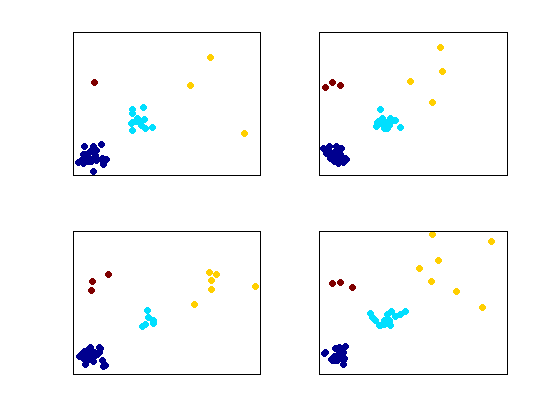
\includegraphics[trim = 4cm 8cm 4cm 8cm, clip, width=5cm]{fig/shared_clustering.pdf}
%\caption{Shared clustering}
\label{default}
\end{center}
\end{figure}
\end{column}
\end{columns}
\end{block}
\end{frame}	


\begin{frame}[t]{Hierarchical Dirichlet Process Inference}
%SMC and MCMC algorithms based on the Polya urn representation exist for hierarchical DP's as well.  
Consider the ``full characterization'' of the posterior predictive distribution of the base level of a DP model
\begin{eqnarray*}
G &\sim& \DP(c,G_0) \\
G_j &\sim& \DP(c,G) \\
\theta_{ij} &\sim& G_j \\
\end{eqnarray*} 
i.e.
\[\theta_{nj} | \theta_{1j}, \ldots, \theta_{n-1,j} =  \frac{1}{n-1+c}\sum_{i=1}^{n-1}\delta_{\theta_{ij}} + \frac{c}{n-1+c}G_j\]

\end{frame}

\begin{frame}[t]{Hierarchical Dirichlet Process Inference}
Now consider $G_j$ as having been similarly marginalized out and represented in the same way

\[\psi_{nj} | \psi_{1j}, \ldots, \psi_{n-1,j} =  \frac{1}{n-1+c}\sum_{i=1}^{n-1}\delta_{\psi_{ij}} + \frac{c}{n-1+c}G\]
Consider the following argument.  If $\theta_{nj} \notin \{\theta_{ij}\}_{i=1}^{n-1}$ then $\theta_{nj}$ must be explained as having been a draw from the base distribution $G_j$
\[\theta_{nj} | \theta_{1j}, \ldots, \theta_{n-1,j} =  \frac{1}{n_j-1+c}\sum_{i=1}^{n_j-1}\delta_{\theta_{ij}} + \frac{c}{n_j-1+c}G_j\]
and correspondingly there must be some $\psi_{ij} = \theta_{ij}$.  This could be one of the existing $\psi$'s or a draw from $G$. This intuition is the basis for MCMC and SMC HDP samplers.  


\end{frame}
\subsection{Pitman-Yor Process}
\input{"../power law slides/powerlaw"}
\subsection{Hierarchical Modeling}
\subsection{Power law}
\label{powerlaw}

\section{Power Law Processes}

\frame[t] {
\frametitle{Power Law Distribution}
A power law distribution is a distribution whose tail falls off as
\[ P(X=x) \propto x^{-\alpha} \]
For some $\alpha > 1$.  The simplest such distribution is the zeta distribution on natural numbers:
\[ f_\alpha(k) = \frac{k^{-\alpha}}{\zeta(\alpha)} \]
and the Pareto distribution on the real line (with small-scale cutoff $x_{min} > 0$):
\[ f_\alpha(x) = \frac{\alpha-1}{x_{min}} \left(\frac{x}{x_{min}}\right)^{-\alpha} \]
}

\frame[t] {
\frametitle{Scale Free Property}
A power law distribution on the real line is {\em scale free} in the sense that, for all scales $k > 0$ and $x > x_{min}$
\[  f_{\alpha}(kx) \propto f_{\alpha}(x) \]
Where the proportionality constant depends only on $k$.
}

\frame[t] {
\frametitle{Power Laws in Nature}
Words in natural language, arranged by frequency \cite{Zipf1965}.
\begin{center}
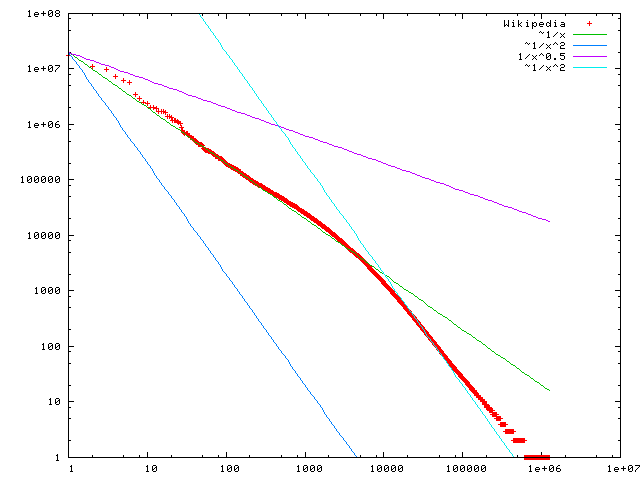
\includegraphics[scale=0.35]{figs/wikipedia-zipf.png} \\
Log-log plot of word frequency in Wikipedia (source: Wikipedia)
\end{center}
}

\frame[t] {
\frametitle{Power Laws in Nature}
Cities arranged by population \cite{Blank2000}.
}

\frame[t] {
\frametitle{Power Laws in Nature}
Earthquakes arranged by magnitude \cite{Gutenberg1955}. \\
\begin{center}
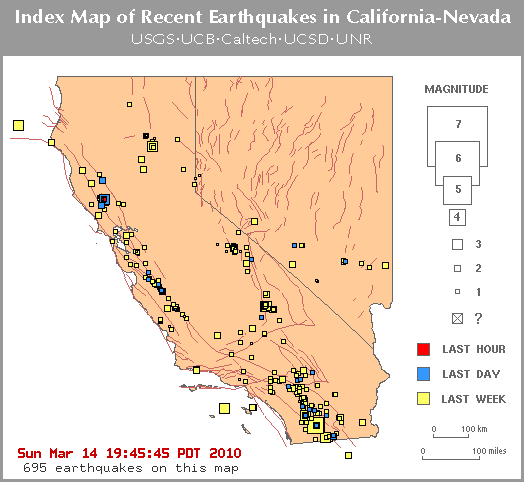
\includegraphics[scale=0.35]{figs/earthquakes.png} \\
(image source: http://quake.usgs.gov/recenteqs/latest.htm)
\end{center}
}

\frame[t] {
\frametitle{Power Laws in Nature}
Power spectra of natural images \cite{Ruderman1994}.
\begin{center}
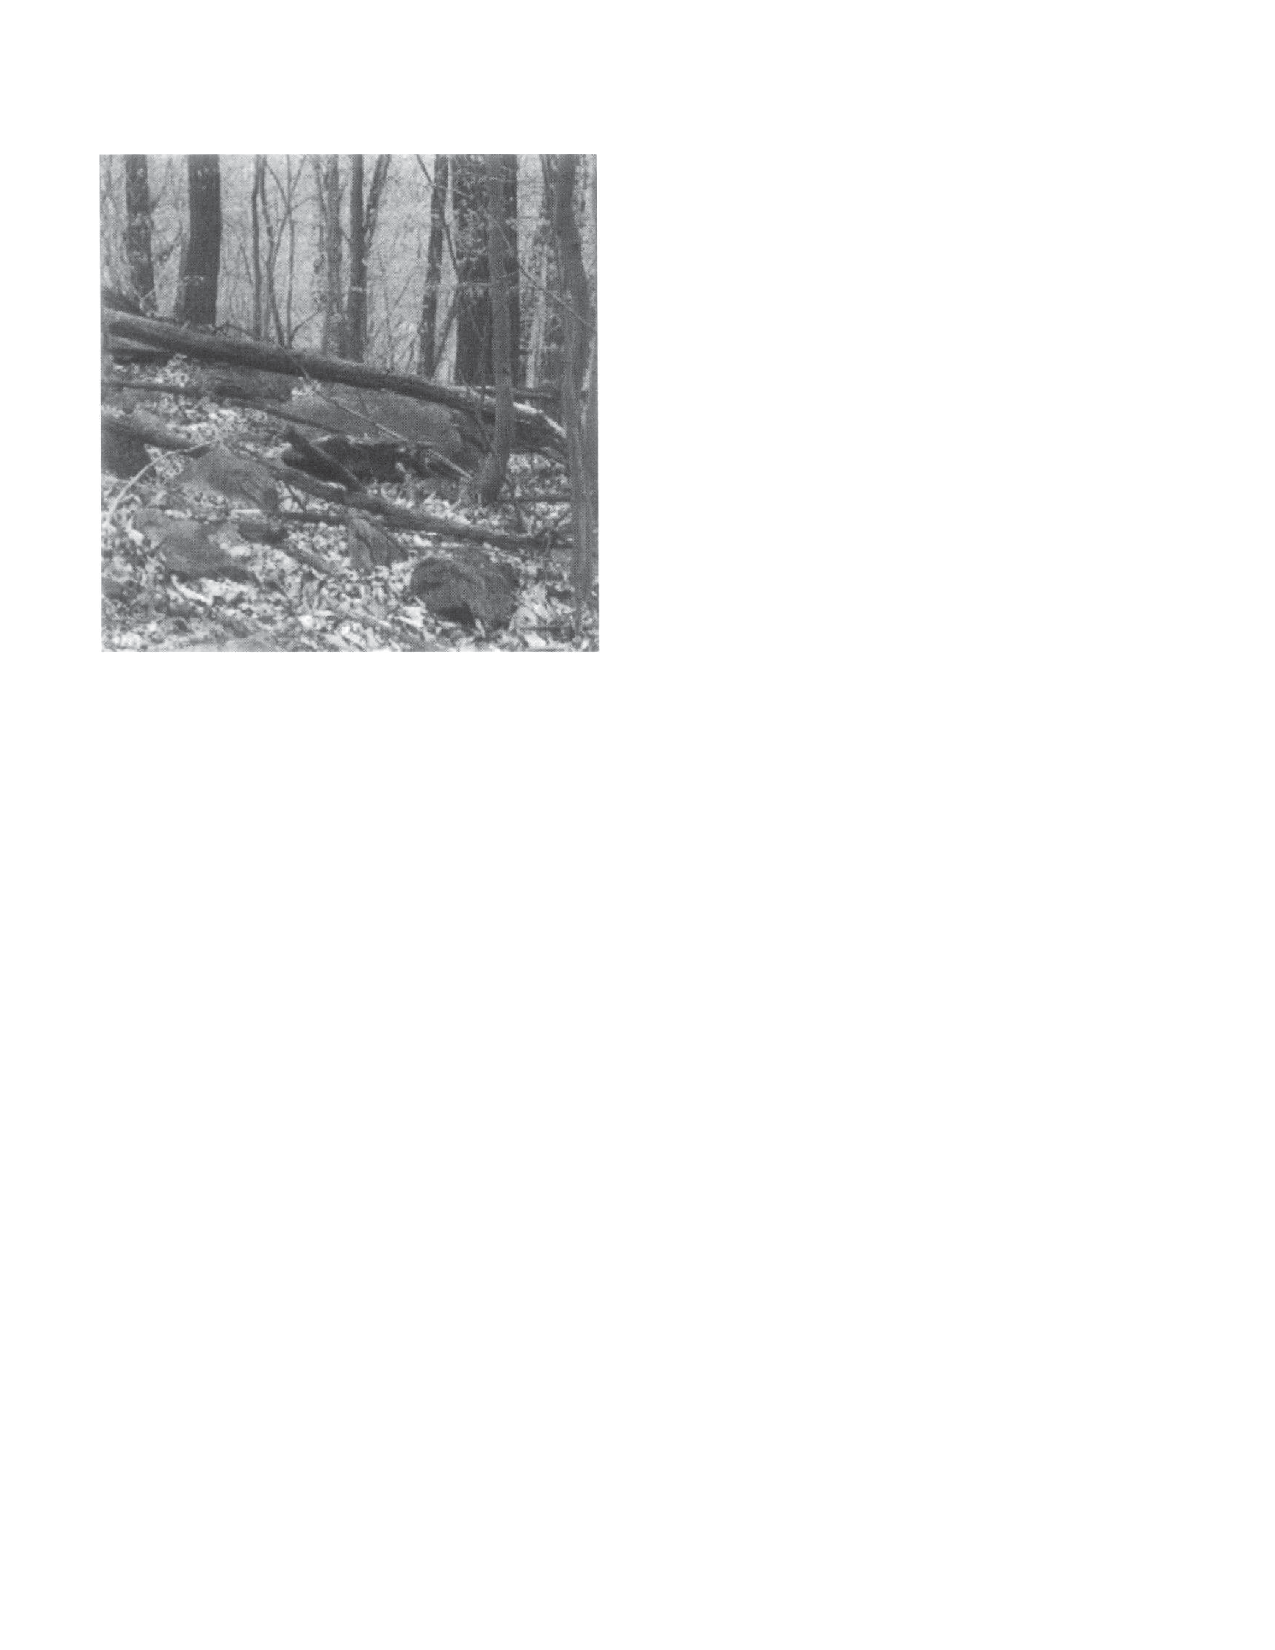
\includegraphics[scale=0.5]{figs/ruderman_bialek_img.pdf}
\hspace*{5 mm}
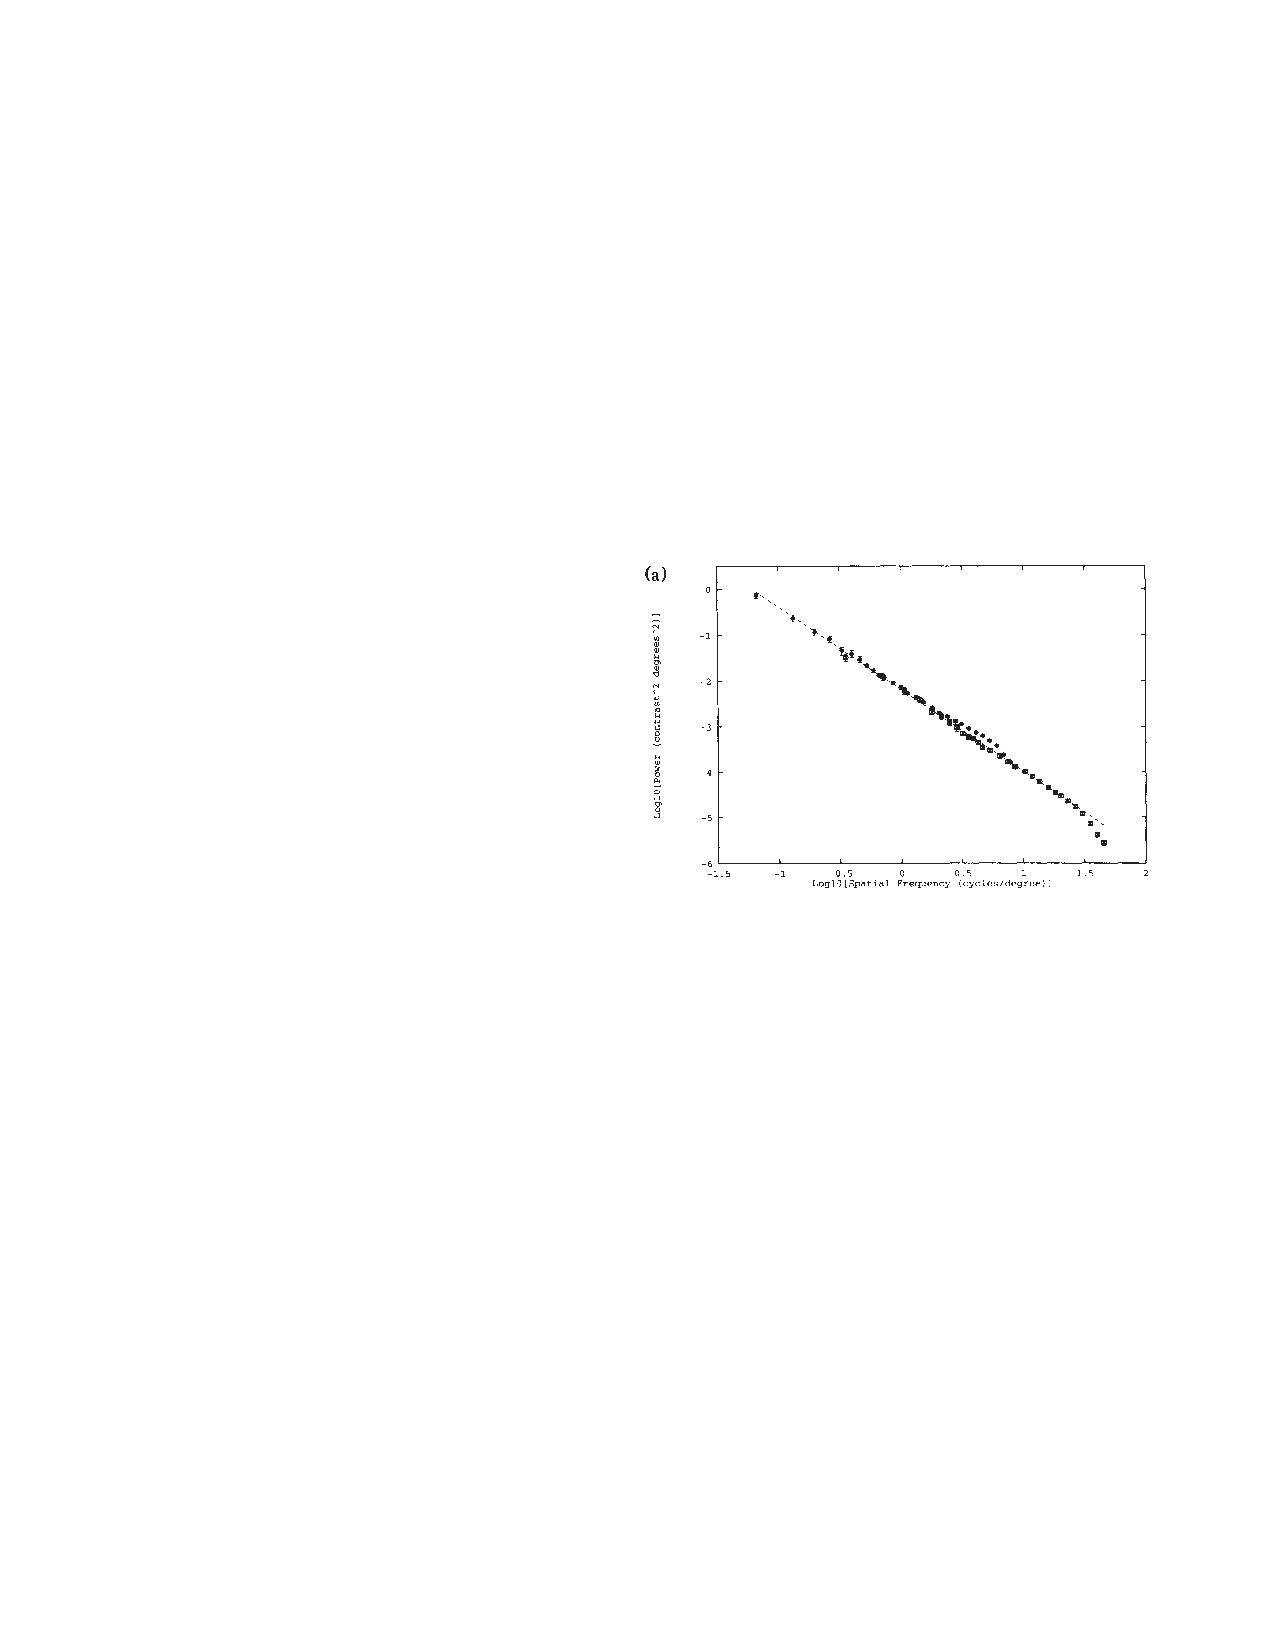
\includegraphics[scale=0.75]{figs/ruderman_bialek_plot.pdf}
\end{center}
}
\section{Example}
\subsection{Sequence Memoizer}






\begin{frame}[t]{Example}
\[
\begin{array}{l}
01001001011011100010000001110100\\
01101000011100100110010101100101\\
00100000011001000110000101111001\\
01110011001000000111010001101001\\
01101101011001010010000001111001\\
01101111011101010111001000100000\\
01101000011000010111001001100100\\
00100000011001000111001001101001\\
01110110011001010010000001101001\\
01110011001000000110011101101111\\
01101001011011100110011100100000\\
01110100011011110010000001100011\\
01110010011000010111001101101000...
\end{array}
\]
\end{frame}	

 \frame[t] {%slide 6
 \frametitle{Sequence Data}
 \begin{itemize}
\item  Natural language processing 
 \begin{itemize}
\item Words, i.e.~the united \_
\item Characters, i.e.~un\_
\item Parts of speech, i.e.~NNV\_
\end{itemize}
\item Compression 
 \begin{itemize}
\item  Bits i.e.~0101000011110001\_
\item  Bytes i.e.~6A7B4ED22100D\_
\end{itemize}
\item Computational biology 
 \begin{itemize}
\item  Nucleotides i.e.~actgtc\_
\item Genes
\item ...
\end{itemize}
\item ...
\end{itemize}

 }
 \frame[t] {%slide 7
 \frametitle{Example Applications}
 \begin{itemize}
 \item Filling in missing segments
 \[ \argmax_{x_1, x_2, \ldots, x_k} P(010010x_1 x_2 x_3 \ldots x_k 010) \]
 \item Predict what comes next in the sequence 
  \[ \argmax_{x_{i+1}} P(010010010x_{i+1}) \]
 \item Determine typicality (clustering)
   \[ \argmax_{k} P_k(010010010) \]

 \end{itemize}
 }
 \frame[t] {%slide 8
 \frametitle{The Sequence Memoizer}
 The sequence memoizer is a regularized (Bayesian\footnote{$P(data,parameters) = P(parameters)P(data|parameters)$}) model of sequences.  \newline
\begin{align}
P(\xbf,\GG) = P(\GG)\prod_{i=0}^{|\xbf|-1}G_{\xbf_{1:i}}(\xbf_{i+1}) \nonumber
\end{align}
The sequence memoizer represents the joint distribution of a sequence in terms of a product of conditional distributions.  If the probability of each
symbol $s$ following each context $\ubf$ is given by a latent variable (distribution) $G_\ubf(s)$ then

\begin{align}
P(\xbf|\GG) = G_{\{\}}(x_{1})G_{x_1}(x_{2})G_{\xbf_{1:2}}(x_{3})\cdots G_{\xbf_{1:(|\xbf|-1)}}(x_{|\xbf|})  \nonumber 
\end{align}

The resulting likelihood is, by definition, a ``joint''\footnote{$P(x_1,\ldots,x_i|\theta) = P(x_1|\theta) P(x_2 | x_1, \theta) P(x_3 | x_1,x_2, \theta) \cdots P(x_i | \xbf_{1:(i-1)}, \theta)$} likelihood.

 }
 \frame[t] {%slide 9
 \frametitle{The Crux of the Matter}
 Can we learn a joint distribution of over sequences of unbounded length given a single training sequence? (!!!) \newline
 
 \quad Obviously not without strong regularization.  \newline
 
 With Bayesian regularization we can do posterior inference of the following flavor
 
 \[P(x_{i+1} | \xbf_{1:i}) = \int G_{\xbf_{1:i}}(x_{i+1}) dP(G_{x_{i+1} }|\xbf_{1:i}) \]
 
 or more recognizably (but less accurately)
 
 \[P(x_{i+1} | \xbf_{1:i}) = \int P(x_{i+1} | \xbf_{1:i}, \GG) P(\GG | \xbf_{1:i}) d\GG \]

 
 
 }
  \frame[t] {%slide 9.5
 \frametitle{Big Picture}
 The sequence memoizer draws on a diverse set of prior art
 \begin{itemize}
 \item A structured prior on the collection of all conditional probability distributions $\GG$, $P(\GG)$
   \begin{itemize}
   \item Hierarchical Pitman Yor process \cite{Teh2006b, Goldwater2006, Teh2006a}
   \end{itemize}
 \item A method for drawing samples from $P(\GG|\xbf)$
    \begin{itemize}
   \item Chinese restaurant franchise sampler \cite{Teh2006b}
   \end{itemize}
 \item A collection of methods for collapsing the the posterior down to a size that grows linearly in the length of the observation sequence. 
    \begin{itemize}
   \item Coagulation and fragmentation operators \cite{Pitman1999, Ho2006}
   \end{itemize}
 \item A set of algorithms to identify the remaining graphical model.
   \begin{itemize}
   \item Suffix tree construction \cite{Weiner1973,Ukkonen1992}
   \end{itemize}
 \end{itemize}
  }
  
 \frame[t] {%slide 10
 \frametitle{History - statistically modeling sequences}
 Take a long sequence
 \begin{quote}
 aaaaagagaaaagaaaagactgggaaaagcgcgcgcgc...
 \end{quote}
 Pick a order for a Markov model (here 2).  Train the Markov model by counting.
 \[G_{aa}(x) = \frac{\#\{aax\}}{\#\{aa\}}, G_{aa}(g) = \frac{4}{13}\]
Problems
 \begin{itemize}
\item Short order Markov models can't capture long range dependencies
\item High order Markov models have many parameters, $O(|\Sigma|^n)$.
 \begin{itemize}
 \item Don't know if $G_{aa}(c) = 0$ or just not enough data seen yet.
 \item $G_{\ubf}(x) = 0$ causes all sorts of inference problems.
 \item Regularization of some form is imperative.
 \end{itemize}
\end{itemize}
 }

\frame[t] {%slide 11
 \frametitle{Reasonable regularizations}
 In many real life sequential generative processes it is reasonable to believe that 
 \[G_{\ubf}(s) \approx G_{\sigma(\ubf)}(s)\]
 Where $\sigma(x_1x_2x_3\ldots x_n) = x_2x_3\ldots x_n$ is the suffix operator.  For example
 \[G_{adl}(y) \approx G_{dl}(y)\]
 or really just 
  \[G_{\ubf} \approx G_{\sigma(\ubf)}\]

 }
\frame[t] {%slide 12
 \frametitle{Language Modeling}
 Smoothing and interpolating n-gram models have utilized this intuition for many years \cite{Kneser1995,MacKay1995,Chen1999, Goldwater2006, Teh2006a} \newline
 
 All of these models can be expressed in forms similar to
 
   \[G_{\ubf}(s) \propto \frac{\#\{\ubf s\}}{\#\{\ubf\}} + \lambda G_{\sigma(\ubf)}(s)\]

 Predictive models for compression also utilize predictive distributions of similar form \cite{Willems2009, Cleary1984}
 }
  \frame[t] {%slide 20
 \frametitle{$O(n^2)$ graphical model}
 \begin{figure}[htbp]
\begin{center}
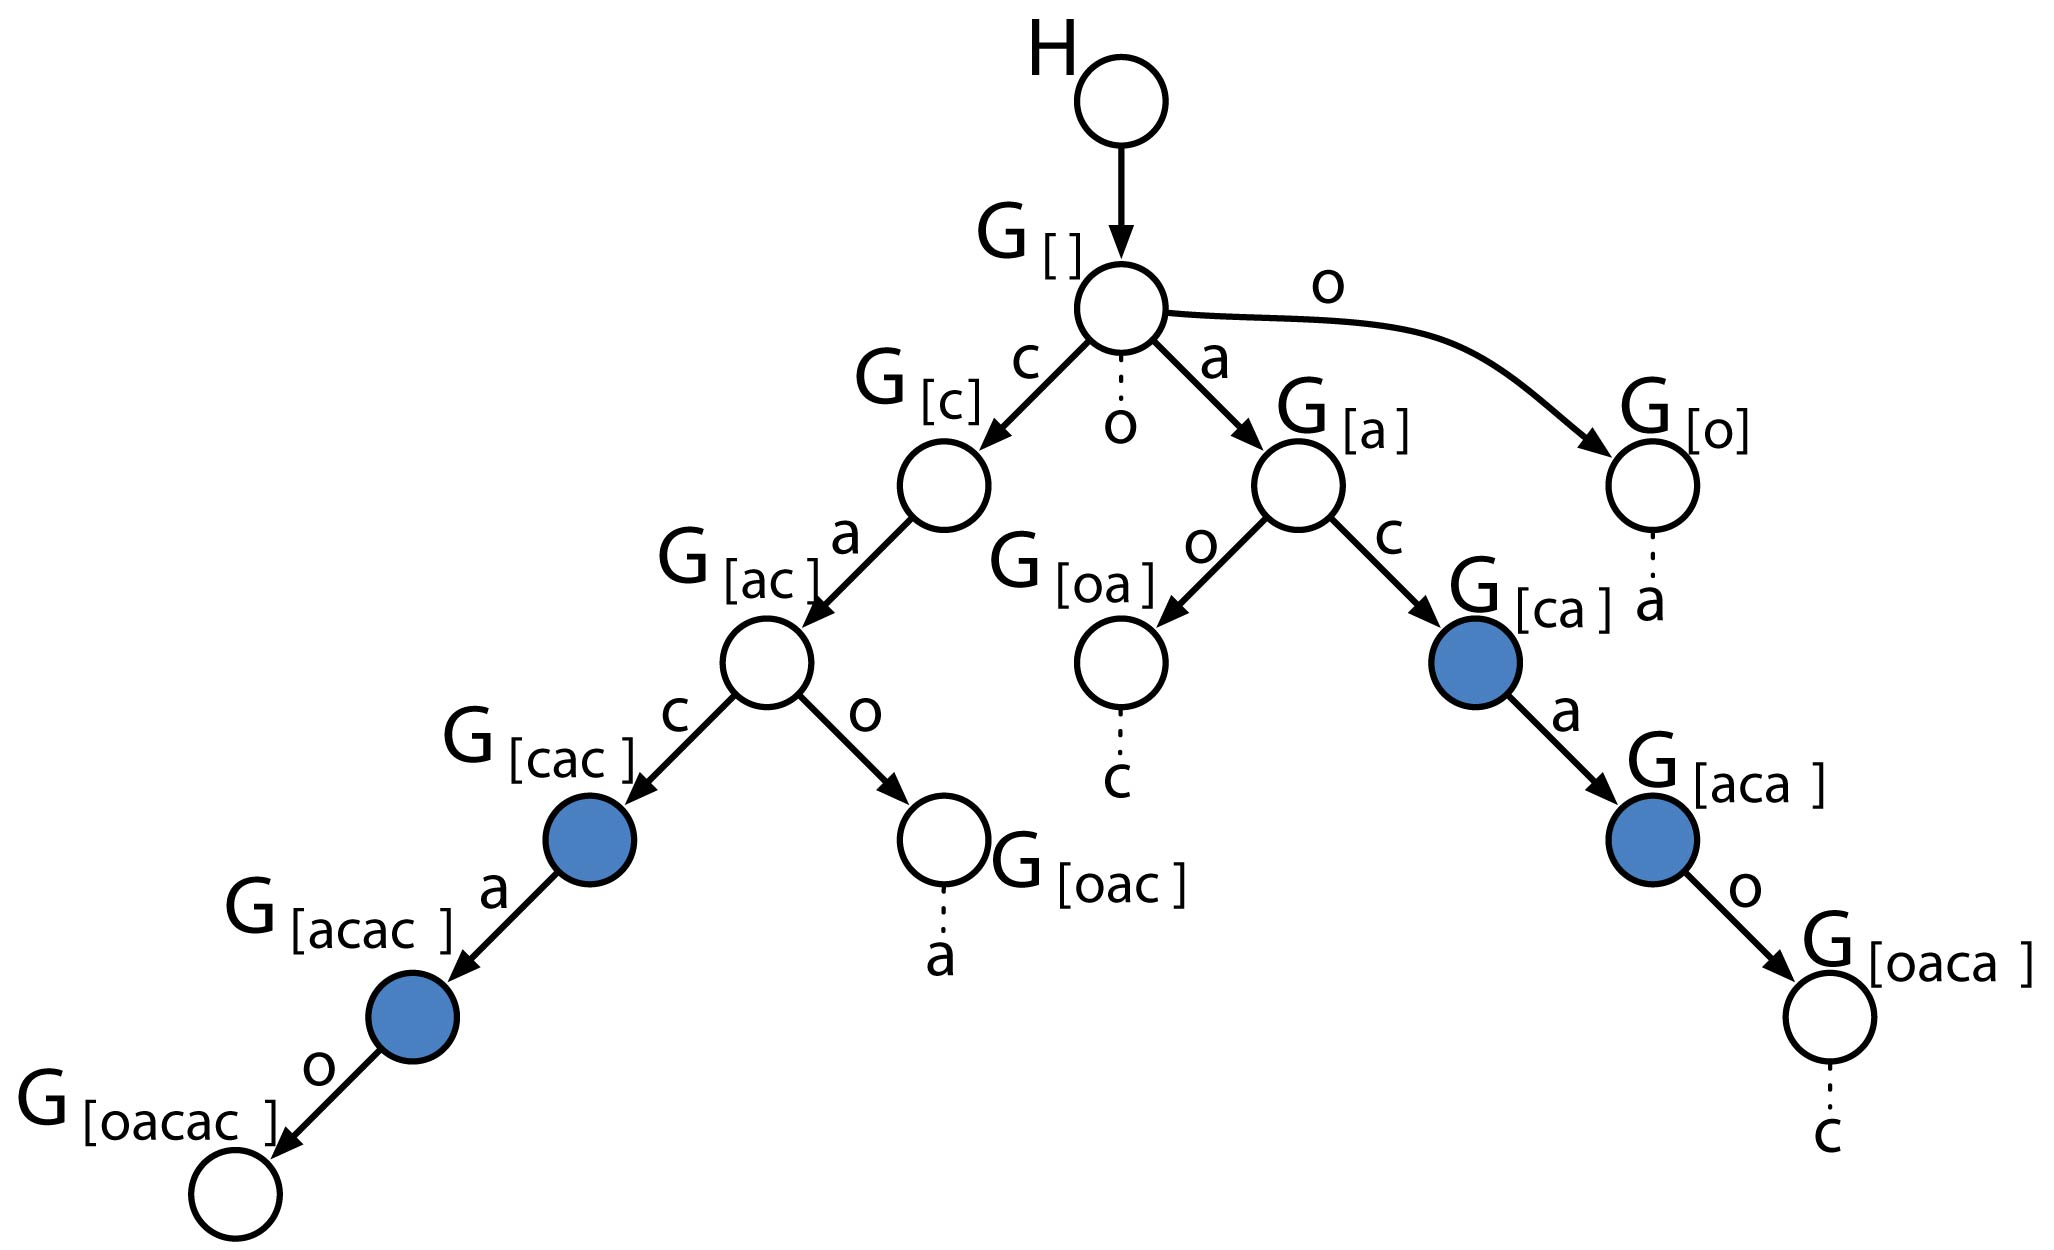
\includegraphics[width=.75\textwidth]{fig/prefix_trie_coloured.pdf}
\caption{Prefix {\em trie} graphical model}
\label{fig: prefix_trie}
\end{center}
\end{figure}
 }
 \frame[t] {%slide 21
\frametitle{$O(n)$ graphical model}
 \begin{figure}[htbp]
\begin{center}
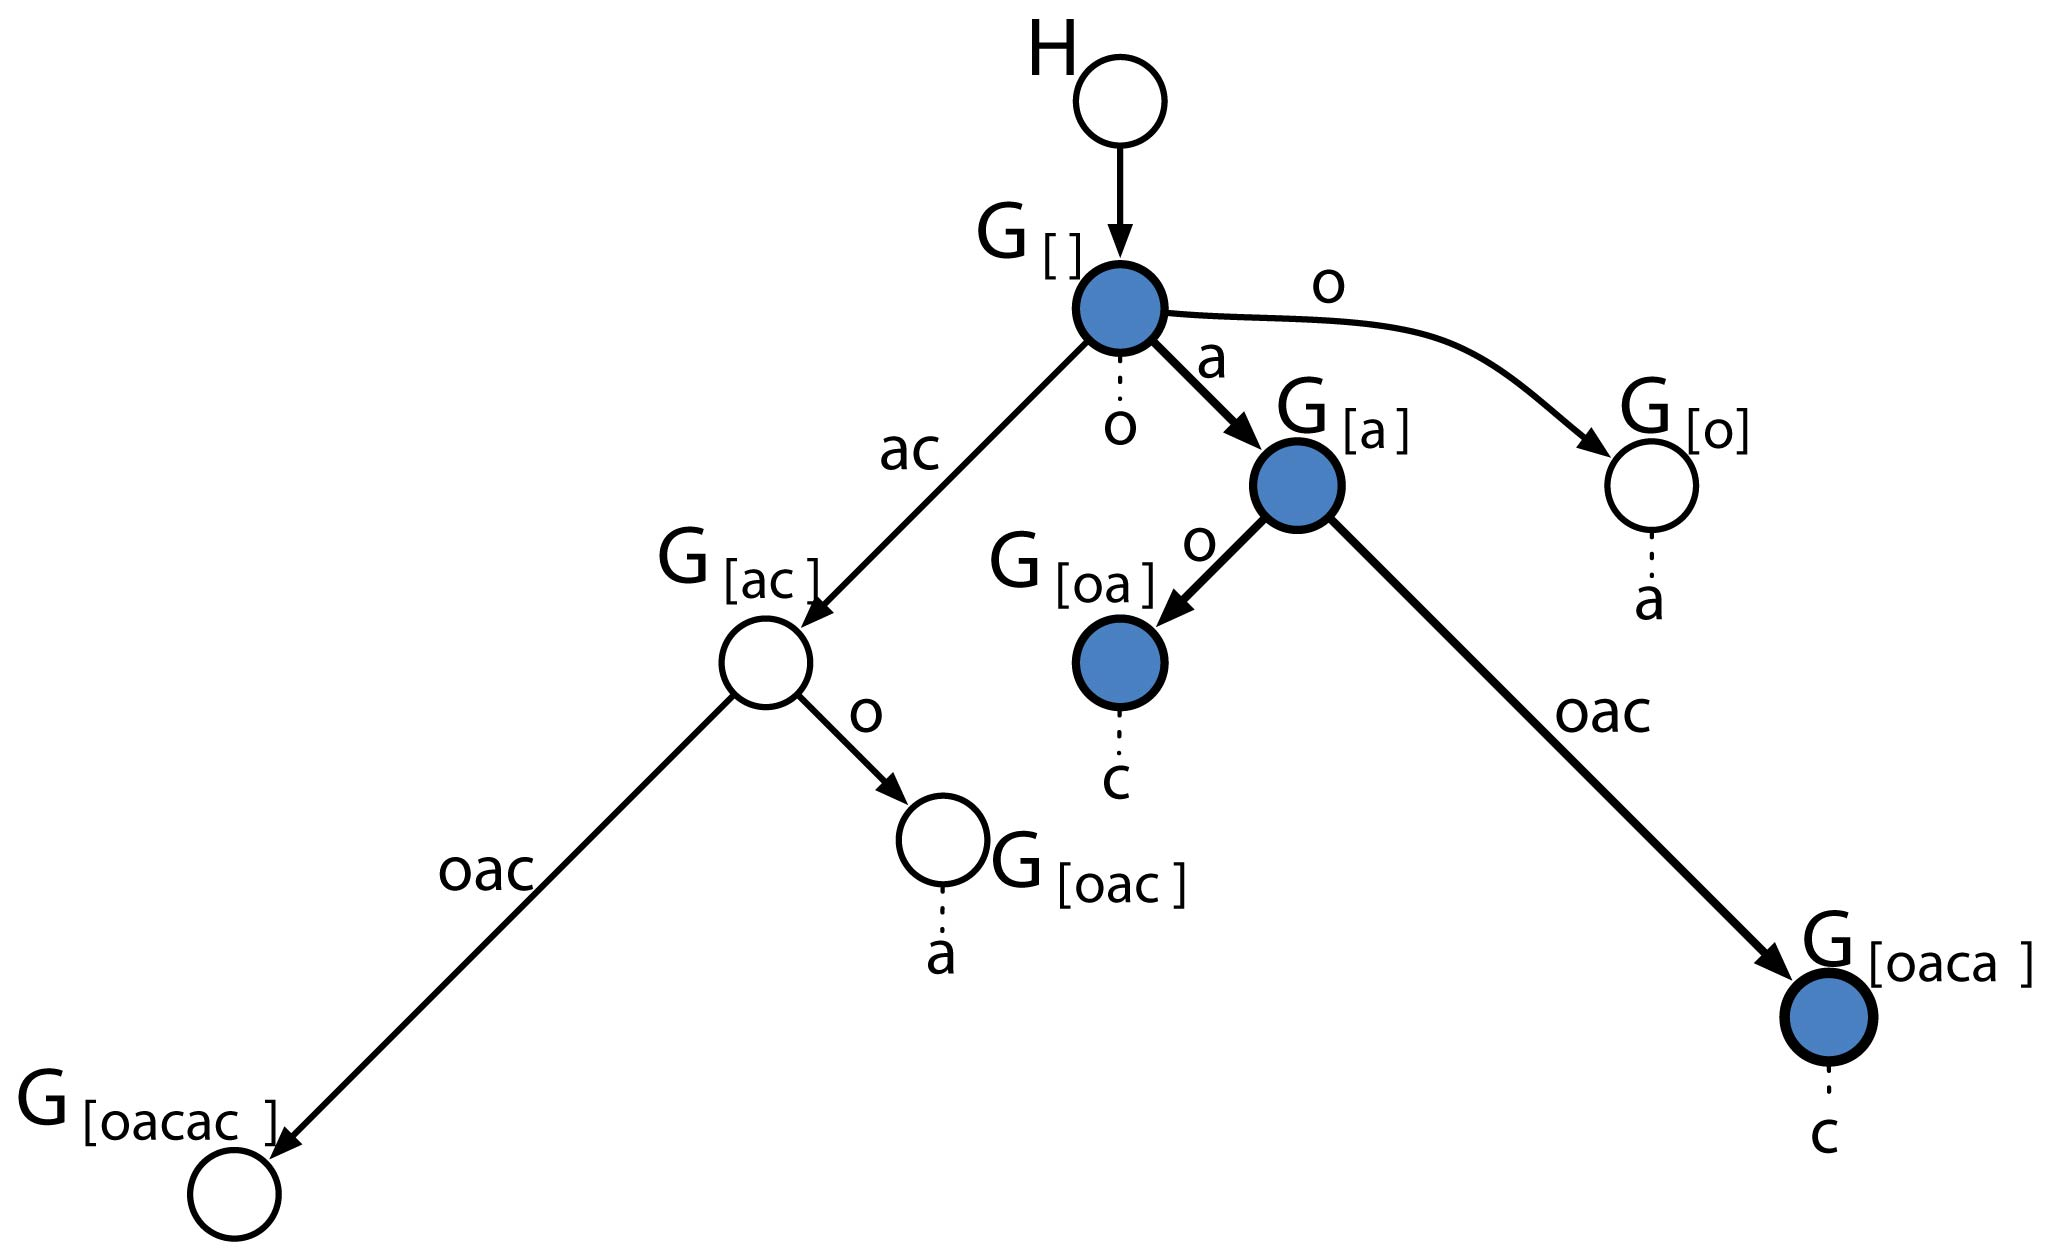
\includegraphics[width=.5\textwidth]{fig/prefix_tree_coloured.pdf}
\caption{Prefix {\em tree} graphical model}
\label{fig: prefix_tree}
\end{center}
\end{figure}
 }
\frame[t] {%slide 22
 \frametitle{}
 }
 \frame[t] {%slide 23
 \frametitle{}
 }
 \frame[t] {%slide 24
 \frametitle{Finite Depth vs.~Infinite Depth - Computational Complexity}
 \begin{figure}[htbp]
\begin{center}
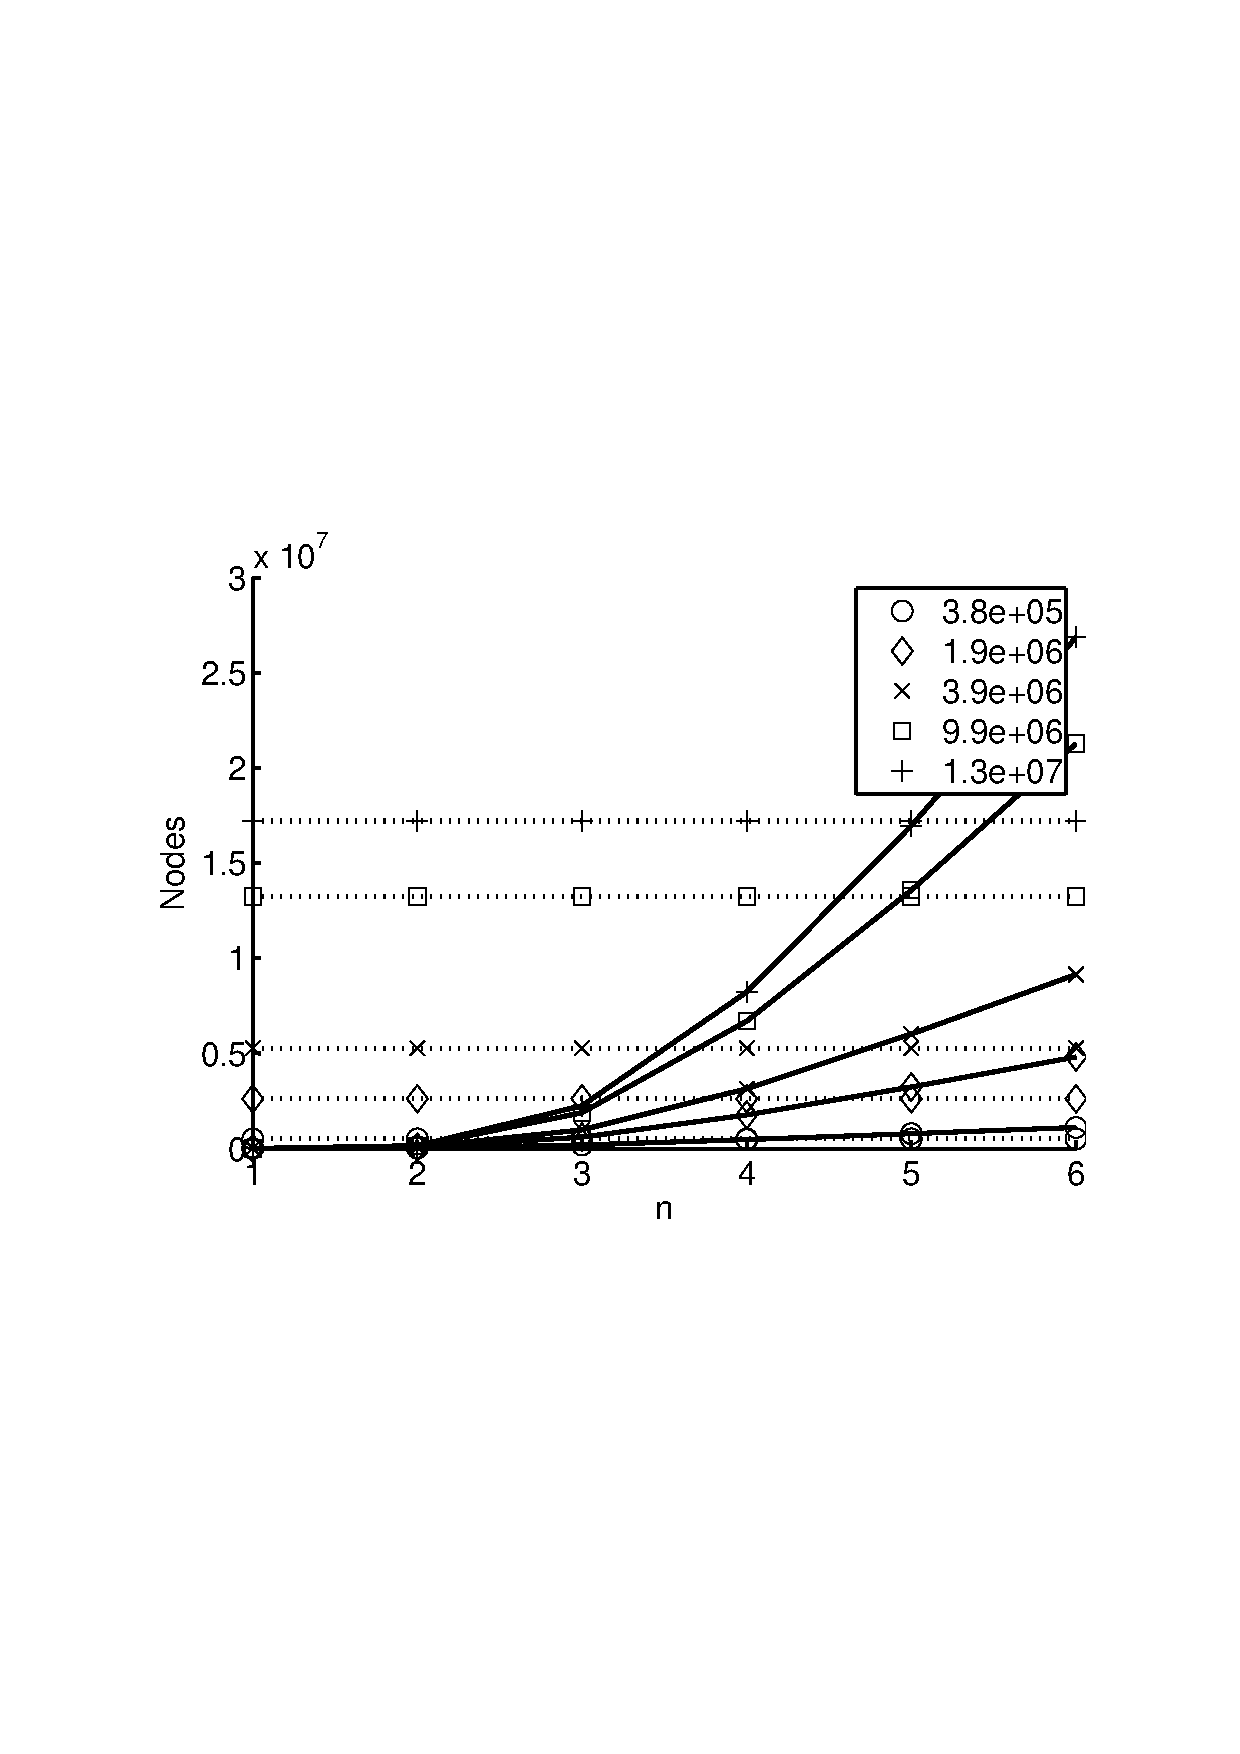
\includegraphics[width=.75\textwidth]{fig/node_counts.pdf}
\caption{Number of nodes vs.~order of Markov model}
\label{fig: node_counts}
\end{center}
\end{figure}
 }
 \frame[t] {%slide 25
 \frametitle{Finite Depth vs.~Infinite Depth - Computational Complexity}
 \begin{figure}[htbp]
\begin{center}
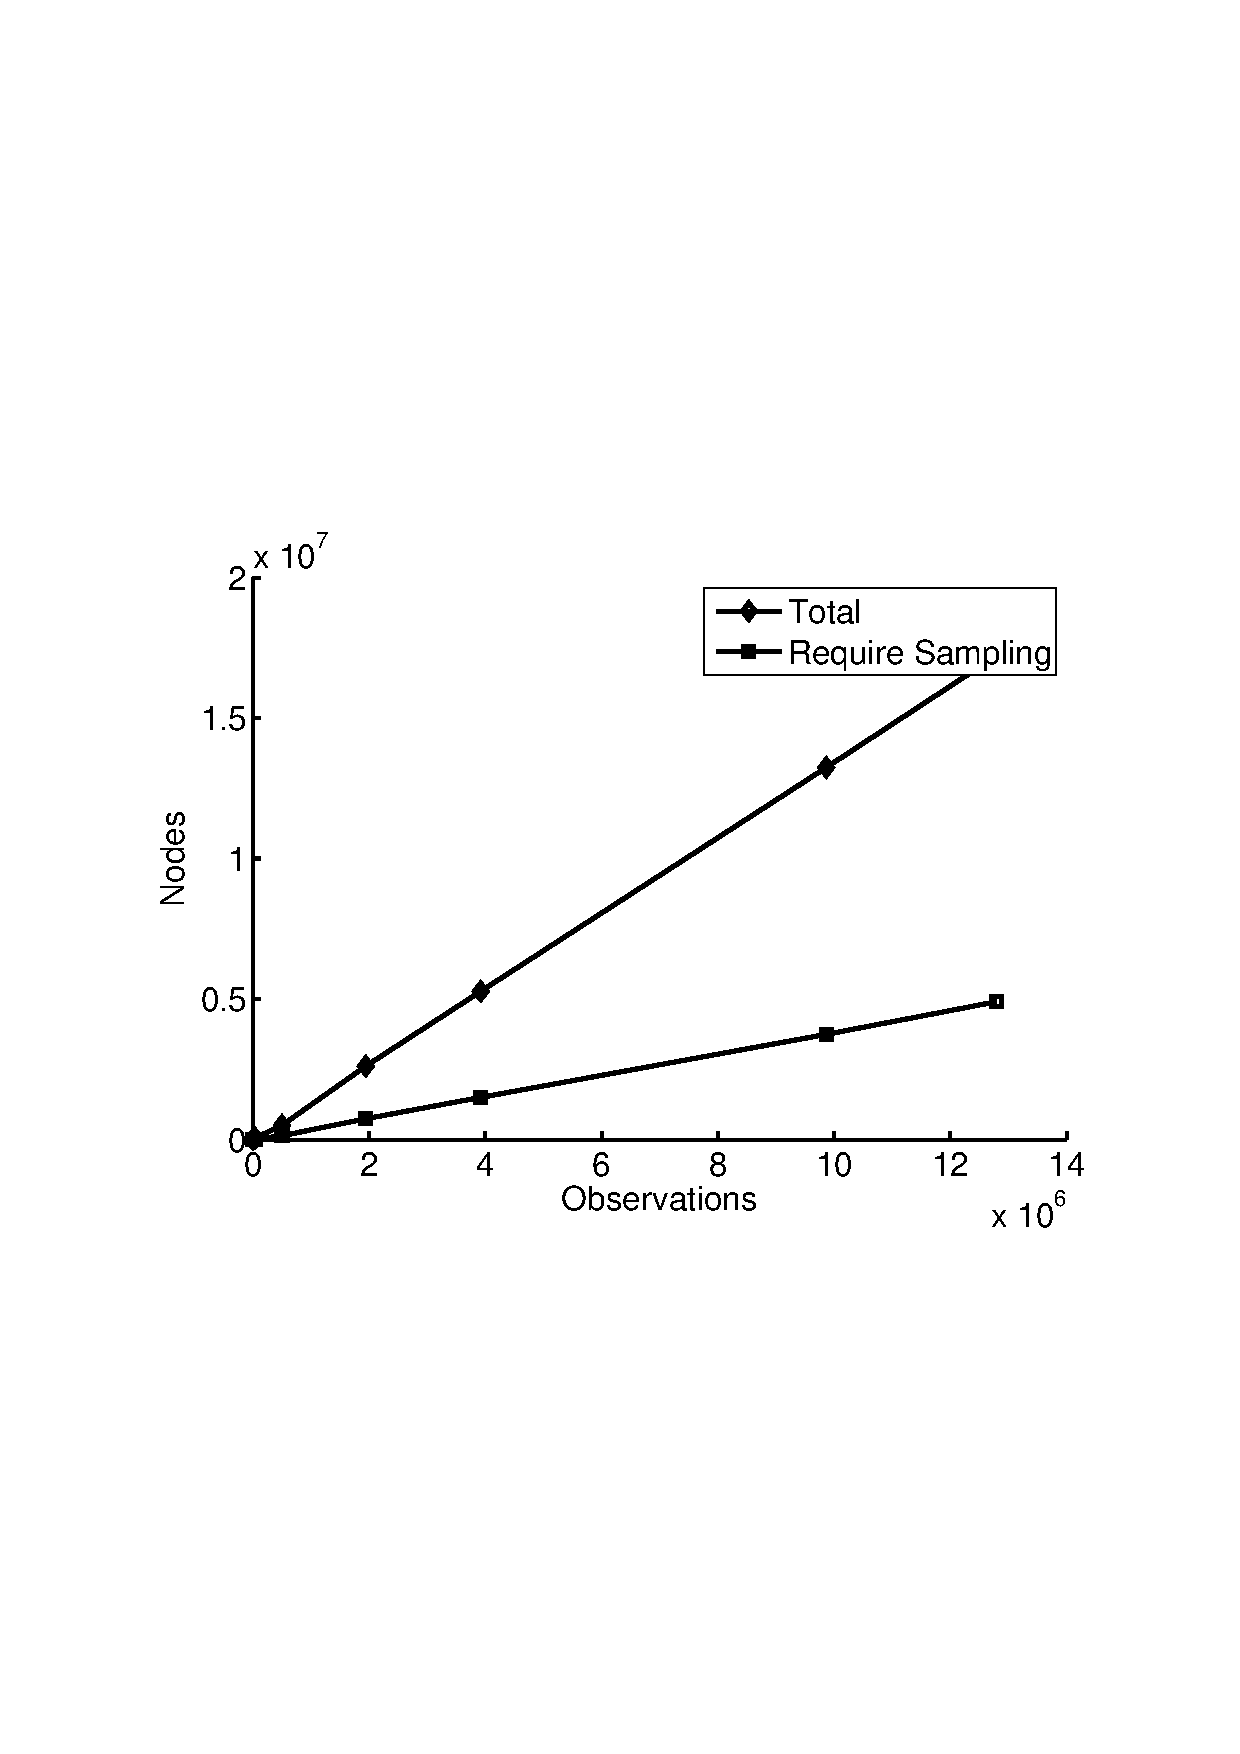
\includegraphics[width=.75\textwidth]{fig/nodes_total_vs_need_sampling.pdf}
\caption{Number of nodes vs.~number of observations}
\label{fig: nodes_total_vs_need_sampling}
\end{center}
\end{figure}
 }
 \frame[t] {%slide 26
 \frametitle{Finite Depth vs.~Infinite Depth - Predictive Power}
 \begin{figure}[htbp]
\begin{center}
\includegraphics[width=.5\textwidth]{fig/fix_size_vary_n_cleaned_coloured.pdf}
\caption{Test perplexity vs.~order of Markov model.}
\label{fig: fix_size_vary_n_cleaned_coloured}
\end{center}
\end{figure}
 }
 \frame[t] {%slide 27
 \frametitle{Finite Depth vs.~Infinite Depth - Predictive Power}
 \begin{figure}[htbp]
\begin{center}
\includegraphics[width=.5\textwidth]{fig/fix_n_vary_size_ap_cleaned_coloured.pdf}
\caption{Test perplexity vs.~number of training observations.}
\label{fig: fix_n_vary_size_ap_cleaned_coloured}
\end{center}
\end{figure}

 }

\section{Discussion}

\frame[t] {%slide 2
 \frametitle{Inspiration}
 ``Prediction and entropy of printed English,'' \citep{Shannon1951}
\begin{quote}
If $[\ldots]$ language is translated into binary digits $[\ldots]$, the entropy H $[\mbox{of the language}]$ is the average number of binary digits required per letter
\end{quote} 
{\begin{center} drppng lttrs dsnt hrt \end{center} }
\begin{quote} $[\ldots]$it appears that, in ordinary literary English, $[\ldots]$ long range statistical effects (up to 100 letters) reduce the entropy to something of the order of one bit per letter
\end{quote}
{\begin{center} d \_ \end{center} }
{\begin{center} the united \_ \end{center} }
{\begin{center} baseball is the national pastime of the united \_ \end{center} }

 }
 \frame[t] {%slide 3
 \frametitle{Inspiration and Reminder}
 Conclusion: lower and upper bound on character-based entropy of English of
$[0.6 < H(English) < 1.3]$ bits per character\footnote{based on a 27 character alphabet, where $log_2(27) \approx 4.75$}\citep{Shannon1951}
 \newline
 
 If $\Sigma$ is a set (an alphabet) and $G$ is a discrete probability distribution over $\Sigma$, (i.e. $\sum_{x\in\Sigma} G(X=x) = 1, 0 < G(x) < 1)$ then you can write the entropy of $G$ as
 
 \[H(G) = -\sum_{x\in\Sigma} G(x) \log_2(G(x))\]
 
 Reminder: entropy is the number of bits per symbol an optimal encoder of a sequence of iid symbols drawn from $G$ would require to losslessly represent the sequence on average. 
 
 }
 \frame[t] {%slide 4
 \frametitle{Crazy Idea}
 \begin{center}Compression $\approx$ intelligence\end{center}
 ``Text Compression as a Test for Artificial Intelligence,''\cite{Mahoney2009} \newline
 
\begin{quote}The Turing test for artificial intelligence is widely accepted, but is subjective, qualitative, non-repeatable, and difficult to implement. An alternative test without these drawbacks is to insert a machine's language model into a predictive encoder and compress a corpus of natural language text. A ratio of 1.3 bits per character or less indicates that the machine has AI.\end{quote}
 }
 \frame[t] {%slide 5
 \frametitle{Of Mouths and Money}
 The (Marcus) Hutter prize \cite{Hutter2006} \newline
 
\begin{quote}Wikipedia is an extensive snapshot of Human Knowledge. If you can compress the first 100MB of Wikipedia better than your predecessors, your (de)compressor likely has to be smart(er). The intention of this prize is to encourage development of intelligent compressors/programs.
 \end{quote}
 \begin{itemize}
\item 50,000 euro in prize money available
\item http://prize.hutter1.net/ 
 \end{itemize}
 }


\section{Thanks}
 \frame[t] {%slide 5
 \frametitle{Collaborators}
 \begin{itemize}
\item Tom Griffiths
\item Yee Whye Teh
\item Jan Gasthaus
\item Nicholas Bartlett
\item David Pfau
\item Sharon Goldwater
 \end{itemize}
 }	
	%\section{References}	

	\bibliographystyle{plainnat}
	\begin{frame}[t,allowframebreaks]{Bibliograpy}

\bibliography{../../papers/uber}
\end{frame}
\end{document}
